\documentclass[11pt]{article}
\usepackage{colacl}
\usepackage{graphicx}
\sloppy



\title{Analysis of Efficient Machine Learning Approaches}
\author
{Sreenath T. Vadakkeveettil}



\begin{document}
\maketitle


\begin{abstract}
This report gives an overview of various Machine Learning algorithms and compare their efficiencies. Also, it gives an insight into various approaches which can be adopted to handle missing data values and confers the impact of discretisation on various machine learning techiques.  
\end{abstract}

\section{Introduction}
Machine learning plays a major role in todays internet era. From amazon's book suggestions to managing traffic in large cities, machine learning is applied in one or other way. Hence it is very essential to have a better understanding of machine learning techniques and algorithms, which can efficiently predict the futuristic problems and find their solutions. This study is performed using WEKA (Waikato Environment for Knowledge Analysis), a machine learning software.     

\section{Handling Missing Values}
The provided dataset being a real world data, many instances have missing attribute values. These can be handled in different ways. In this project, this has been handled using weka's unsupervised attribute filter named ReplaceMissingValues. This filter replaces the missing attribute values by means and modes for numeric and nominal attributes respectively. 

Another promising approach is to use a K nearest neighbour methodology in which the instances which are most similar to the instance with missing value is computed using a distance function and then the mean or mode of the attribute value of those instances are considered. 

According to Section V-B of  \newcite{missing2013}, this method could improve the efficiency of the classifier when compared to those which handled missing values using normal ReplaceMissingValues filter in weka. However, the analysis in this report is based on handling using ReplaceMissingValues.  

\section {Analysis using various classifiers}
Various Classifiers like K-nearest neighbour, decision trees, etc were deployed to identify the ideal classifier using the training set and development set. Only relevant, the ones with higher accuracy is discussed in the sub sections. The analysis provided below is based on the classification of development data by the classifier modelled using training data. Also, other useful details like confusion matrix has been omitted from report in order to utilize the word count. 

\subsection{J48}
J48 is an opensource implementation of C4.5 algorithm in weka \newcite{wikiJ4814}. This algorithm is used to generate decision trees using the concept of information entropy. Table~\ref{table-1} depicts the percentage of correct and incorrect instances classified.

\begin{table}[h]
 \begin{center}
  %\tabcolsep=0.11cm
\begin{tabular}{|l|l|}

	\hline
     Metric & Value  \\
     \hline\hline
     Correctly Classified Instances & 85.37\% \\
	 Incorrectly Classified Instances & 14.63\% \\
	 Mean Absolute Error& 0.2044 \\
     \hline
     
 \end{tabular}
\caption{Evaluation metrics using J48 algorithm}\label{table-1}
 \end{center}
\end{table}

But according to \newcite{JRM95}, there is high impact on the accuracy of the classification when supervised discretization of data is performed before applying these classification algorithms.   

\begin{table}[h]
 \begin{center}
  %\tabcolsep=0.11cm
\begin{tabular}{|l|l|}

	\hline
     Metric & Value  \\
     \hline\hline
     Correctly Classified Instances & 86.42\% \\
	 Incorrectly Classified Instances & 13.58\% \\
	 Mean Absolute Error& 0.1924 \\
     \hline
     
 \end{tabular}
\caption{Evaluation metrics using J48 algorithm on discretised data}\label{table-2}
 \end{center}
\end{table}

Table~\ref{table-2} shows the metrics evaluated using J48 algorithm when applied on supervised dicretised data using Filter Classifier in weka. This clearly indicates the impact of supervised discretisation on classification accuracy. (Procedure used is discussed in README file)

\subsection{Naive Bayes}
Naive Bayes Classifier is a probabilistic classifier which works on the assumption that attributes are conditionally independent given the class variable. One advantage of this approach is that it needs only a small amount of training data to classify efficiently. \newcite{Naive2014}

\begin{table}[h]
 \begin{center}
  %\tabcolsep=0.11cm
\begin{tabular}{|l|l|}

	\hline
     Metric & Value  \\
     \hline\hline
     Correctly Classified Instances & 83.61\% \\
	 Incorrectly Classified Instances & 16.39\% \\
	 Mean Absolute Error& 0.1809 \\
     \hline
     
 \end{tabular}
\caption{Evaluation metrics using Naive Bayes Classifier}\label{table-3}
 \end{center}
\end{table}

Refer Table~\ref{table-3} for evaluation metrics using Naive bayes classifier

\subsection{Support Vector Machines}
Support Vector machine represents each of the instances of training data in a n dimensional vector space so that there is a clear gap between the instances belonging to separate classes. Then the instances in test data is also mapped into same space and is predicted to belong to a category based on which side of the gap they fall. \newcite{svm2014}. Refer Table ~\ref{table-4}

\begin{table}[h]
 \begin{center}
  %\tabcolsep=0.11cm
\begin{tabular}{|l|l|}

	\hline
     Metric & Value  \\
     \hline\hline
     Correctly Classified Instances & 84.99\% \\
	 Incorrectly Classified Instances & 15.01\% \\
	 Mean Absolute Error& 0.1501 \\
     \hline
     
 \end{tabular}
\caption{Evaluation metrics using Support Vector Machine Classifier}\label{table-4}
 \end{center}
\end{table}

\subsection{NBTree Classifier}
As discussed in \newcite{Kohavi96}, NBTree is a hybrid of decision tree classifiers and naive bayes classifiers where the decision-tree nodes contain univariate splits as regular decision-trees, but the leaves contain Naive-Bayesian classifiers. The classifier using this algorithm performs much better than normal decision tree algorithms as well as naive bayesian classifiers. Table~\ref{table-5} illustrates the metrics evaluated using this approach

\begin{table}[h]
 \begin{center}
  %\tabcolsep=0.11cm
\begin{tabular}{|l|l|}

	\hline
     Metric & Value  \\
     \hline\hline
     Correctly Classified Instances & 85.93 \% \\
	 Incorrectly Classified Instances & 14.07 \% \\
	 Mean Absolute Error&  0.1696 \\
     \hline
     
 \end{tabular}
\caption{Evaluation metrics using NBTree Classifier}\label{table-5}
 \end{center}
\end{table}

By comparing its correctly classified instances with that of J48 and Naive Bayes, it can be seen that NBTrees accuracy is higher than the former. However, its value 85.93\% is less than 86.42\% obtained by J48 when applied on discretised data. Hence NBTree was applied on a supervised discretised data in order to identify the impact of discretisation on this classifier.  

\begin{table}[h]
 \begin{center}
  %\tabcolsep=0.11cm
\begin{tabular}{|l|l|}

	\hline
     Metric & Value  \\
     \hline\hline
     Correctly Classified Instances & 86.58 \% \\
	 Incorrectly Classified Instances & 13.42 \% \\
	 Mean Absolute Error& 0.167 \\
     \hline
     
 \end{tabular}
\caption{Evaluation metrics using NBTree Classifier on discretised data}\label{table-6}
 \end{center}
\end{table}

From Table~\ref{table-6}, it is clear that this model is the best classifier among the ones analysed so far since its \% of correctly classified instances are much more than the ones obtained by other classifiers. Hence this model will be used for classifying the test data. 

\section{Classification of test dataset}
Test data set has been classified in two different ways in this project. One using the adultTrain.arff as Training set and secondly by combining data in adultTrain.arff and adultDevelopment.arff. By comparing the output, it is noticed that there are small differences in the class identified in some instances. I assume the second approach would yield a better classification output since the training set has more data which would help the classifier to approprately determine the class. Both these results will be submitted along with README file.

\section{Problem addressed}
Using the census data provided from 1994, I tried to solve the original problem discussed in the project spec. Whether I can get rich as soon as I graduate. Using a new test dataset with one instance which best describes my qualifications once I graduate, I tried to classify whether a person with same qualification as me in 1994 belong to greater than 50K or less than or equal to 50K salary class. Although, some of the details are not accurate like capital-gain, capital-loss, etc, according to this classifier, the person belongs to the latter class i.e, less than or equal to 50K. 

\section{Sub Problem Considered}
Do we live in a world where genders are treated equally ?
This is an analysis based on one attribute, i.e gender. By filtering the gender to have only value. It can be seen that according to training data, 6662 males have more than 50K as salary out of 21790. i.e 30.57\%. But in case of females, only 1179 females have more than 50K salary out of 10771. i.e 10.94\%. Hence it can be deduced that females are comparatively earning less than males or in other words, less percentage of females are working in sectors which gives higher salary.

\begin{figure}[h]
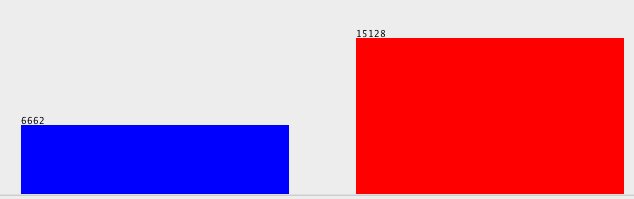
\includegraphics[width=7cm]{Screen_Shot_2014-06-01_at_11_39_19_AM.png}
\caption{Salary distribution in case of males}
\end{figure}

\begin{figure}[h]
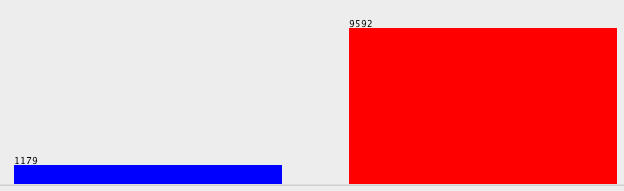
\includegraphics[width=7cm]{Screen_Shot_2014-06-01_at_11_58_00_AM.png}
\caption{Salary distribution in case of females}
\end{figure}

\section{Conclusions}
The analysis done in this project shows that NBTree machine learning algorithm performs much better in classifying compared to other classifiers analysed. This report also discusses various promising approaches in handling missing attribute values mainly the K nearest neighbour approach mentioned in section 2. Also, it emphasises the impact of supervised discretisation on the classifier model. Hence it can be concluded that the machine learning not only depend on the algorithm chosen, but also on the way the data is handled. 


\bibliographystyle{acl}
\bibliography{sample}

\end{document}
